\documentclass[12pt,class=report,crop=false]{standalone}
\usepackage[screen]{../python}

\pagestyle{empty}

\begin{document}

% Commande spécifique
\newcommand{\badletter}[1]{\underline{\textcolor{red}{#1}}}



%====================================================================
\chapitre{Listes I}
%====================================================================


\section*{Construction d'une liste}

Une \defi{liste}\index{liste} est une suite d'éléments. 

\bigskip
\begin{itemize}
  \item \ci{[5,-7,12,99]}
  \item \ci{["Mars","Avril","Mai"]} 
  \item \ci{[3.14,"pi",10e-3,"x",True]}
\end{itemize}

\bigskip

\begin{itemize}
  \item Une liste se définit par des éléments entre crochets :
  \begin{itemize}
    \item \ci{liste1 = [5,4,3,2,1]} 
    \item \ci{liste2 = ["Vendredi","Samedi","Dimanche"]} 
    \item \ci{liste3 = []} la liste vide (très utile pour la compléter plus tard  !).
  \end{itemize}
\end{itemize}

\newpage

\section*{Accéder à un élément}

 Pour obtenir un élément de la liste, il suffit d'écrire 
 
 \centerline{\ci{liste[i]}} 
 
 où $i$ est le rang de l'élément souhaité. 

\bigskip
  
  \textbf{Attention.} On commence à compter à partir du rang $0$ ! 
  
\bigskip
  
  
  Par exemple après l'instruction \ci{liste = ["A","B","C","D","E","F"]} alors  
  \begin{itemize}
    \item \ci{liste[0]} renvoie \ci{"A"}
    \item \ci{liste[1]} renvoie \ci{"B"}
    \item \ci{liste[2]} renvoie \ci{"C"}
    \item \ci{liste[3]} renvoie \ci{"D"}
    \item \ci{liste[4]} renvoie \ci{"E"}
    \item \ci{liste[5]} renvoie \ci{"F"}                   
  \end{itemize}  
  
  \medskip
  
 \myfigure{0.6}{
  \tikzinput{fig-listes-1}
}  

\newpage


\section*{Ajouter un élément}

 Pour ajouter un élément à la fin de la liste, il suffit d'utiliser la commande 
  
 \centerline{\ci{maliste.append(element)}} 
    
  \bigskip
  \bigskip 

  \begin{itemize}
    \item  \ci{premiers = [2,3,5,7]},
    \item puis \ci{premiers.append(11)} rajoute $11$ à la liste, 
    \item puis \ci{premiers.append(13)} alors maintenant la liste \ci{premiers} vaut \ci{[2,3,5,7,11,13]}.
  \end{itemize}  
  
\newpage

\section*{Une construction}

 Voici comment construire la liste qui contient les premiers carrés.
 
  \bigskip
  \bigskip 
  
   \begin{center}
  \begin{minipage}{0.9\textwidth}
\begin{lstlisting}
liste_carres = []          # On part d'un liste vide
for i in range(10):
    liste_carres.append(i**2)   # On ajoute un carré
\end{lstlisting}
  \end{minipage}
  \end{center}  
\`A la fin \ci{liste_carres} vaut :\\
\centerline{\ci{[0, 1, 4, 9, 16, 25, 36, 49, 64, 81]}}   
          

\newpage

 \section*{Parcourir une liste} 
 
\begin{itemize}
  \item \textbf{Longueur d'une liste.}  \ci{len(liste)}
  
  \begin{itemize}
  \item La liste \ci{[5,4,3,2,1]} est de longueur $5$, 
  \item la liste \ci{["Vendredi","Samedi","Dimanche"]} de longueur $3$, 
  \item la liste vide \ci{[]} de longueur $0$.
  \end{itemize}
  
   \bigskip

  
  \item \textbf{Parcourir une liste.} 
	Voici la façon la plus simple de parcourir une liste (et ici d'afficher chaque élément) :
\index{for@\ci{for}}\index{boucle!pour}
\begin{lstlisting}
for element in liste:
    print(element)
\end{lstlisting}

  \bigskip 
  
  \item \textbf{Parcourir une liste (bis).} 
  Parfois on a besoin de connaître le rang des éléments. Voici une autre façon de faire (qui affiche ici le rang et l'élément).
\begin{lstlisting}
n = len(liste)
for i in range(n):
    print(i,liste[i])
\end{lstlisting}  

  \bigskip 
  
\item Pour obtenir une liste à partir de \ci{range()} il faut écrire :\\
\centerline{\ci{list(range(n))}}
\end{itemize}


\newpage


\section*{Concaténer}

\begin{itemize}
  \item \textbf{Concaténer deux listes.}
  Si on a deux listes, on peut les fusionner par l'opérateur \og{}\ci{+}\fg{}. 
  
  Exemple.
  \ci{liste1 = [4,5,6]} et \ci{liste2 = [7,8,9]}  \\
  \centerline{\ci{liste1 + liste2} \quad vaut \quad \ci{[4,5,6,7,8,9]}.}
  
  \bigskip
  \bigskip   
    
  \item \textbf{Ajouter un élément à la fin.}
  
  \centerline{\ci{liste = liste + [element]}}
  
  Exemple. \ci{[1,2,3,4] + [5]} vaut \ci{[1,2,3,4,5]}.
     
  C'est une méthode alternative à \ci{liste.append(element)}.
 
   \bigskip
  \bigskip 
    
  \item \textbf{Ajouter un élément au début.}
  
  \centerline{\ci{liste = [element] + liste}}
  

  Exemple \ci{[5] + [1,2,3,4]} vaut \ci{[5,1,2,3,4]}. 
\end{itemize}
  
\newpage


\section*{Trancher des listes}

\index{liste!sous-liste} On peut extraire d'un seul coup toute une partie de la liste :

\centerline{\ci{liste[a:b]}}

renvoie la sous-liste des éléments de rang $a$ à $b-1$.
  

  \bigskip   
  
 \myfigure{0.4}{
  \tikzinput{fig-listes-3}
}  
  
  \bigskip
  \bigskip    
  
    Par exemple si \ci{liste = ["A","B","C","D","E","F","G"]} alors  
  \begin{itemize}
    \item \ci{liste[1:4]} renvoie \ci{["B","C","D"]}
    \item \ci{liste[0:2]} renvoie \ci{["A","B"]}
    \item \ci{liste[4:7]} renvoie \ci{["E","F","G"]}
  \end{itemize} 
  
  \bigskip   
  
  Il faut encore une fois faire attention à ce que le rang d'une liste commence à $0$ et que le tranchage \ci{liste[a:b]} s'arrête au rang $b-1$.
  
  

\newpage

\section*{Manipulation des listes}

\begin{itemize}
  \item \textbf{Inverser une liste.}\index{liste!inverser} Voici trois méthodes :\index{reverse@\ci{reverse/reversed}}
\begin{itemize}
  \item \ci{maliste.reverse()} modifie la liste sur place (c'est-à-dire que \ci{maliste} est maintenant renversée, la commande ne renvoie rien) ;
  \item \ci{list(reversed(maliste))} renvoie une nouvelle liste ;
  \item \ci{maliste[::-1]} renvoie une nouvelle liste. 
\end{itemize} 

   \bigskip
  \bigskip 

  \item \textbf{Supprimer un élément.}  La commande \ci{liste.remove(element)}\index{liste!supprimer}\index{remove@\ci{remove}} supprime la première occurrence trouvée (la liste est modifiée). Par exemple avec \ci{liste = [2,5,3,8,5]} la commande \ci{liste.remove(5)} modifie la liste qui maintenant vaut \ci{[2,3,8,5]} (le premier $5$ a disparu).
  
  \bigskip
  \bigskip 
  
   \item \textbf{Supprimer un élément (bis).}  La commande \ci{del liste[i]}\index{del@\ci{del}} supprime l'élément de rang $i$ (la liste est modifiée).
  
\end{itemize}


\newpage

\section*{Tri}

\index{liste!trier}
\index{sorted@\ci{sort/sorted}} 
 
  \begin{fonctionpython}[\ci{python : sorted()}]
    Usage : \ci{sorted(liste)}\\
    Entrée : une liste  \\
    Sortie : la liste ordonnée des éléments
  
  \medskip
     
   Exemple : \ci{sorted([13,11,7,4,6,8,12,6])} renvoie la liste \ci{[4,6,6,7,8,11,12,13]}.

  \end{fonctionpython}  
  
  Attention ! Il existe aussi une méthode \ci{liste.sort()} qui modifie la liste sur place.

\newpage

\section*{Visualiser une liste}

Avec le module \ci{matplotlib} il est très facile de visualiser les éléments d'une liste de nombres.

\begin{center}
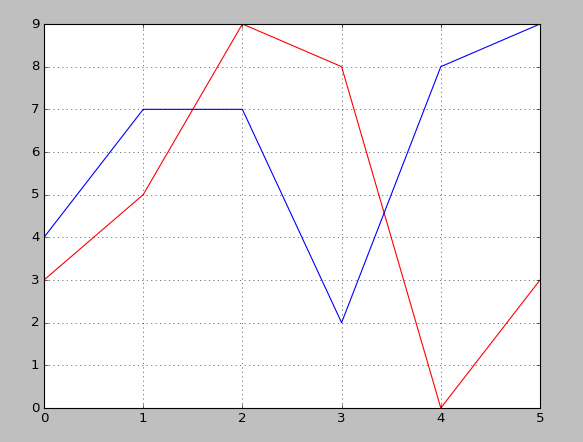
\includegraphics[scale=0.45]{ecran-liste-cours-visualisation}
\end{center}

\begin{lstlisting}
import matplotlib.pyplot as plt

liste1 = [3,5,9,8,0,3]
liste2 = [4,7,7,2,8,9]

plt.plot(liste1,color="red")
plt.plot(liste2,color="blue")
plt.grid()
plt.show()
\end{lstlisting}


%\newpage
%
%\emph{Explications.}
%\begin{itemize}
%  \item Le module s'appelle \ci{matplotlib.pyplot} et on lui donne le nouveau nom plus simple de \ci{plt}.
%  
%  \item Attention ! Le module \ci{matplotlib} n'est pas toujours installé par défaut avec \Python.
%  
%  \item \ci{plt.plot(liste)}\index{plot@\ci{plot}} trace les points d'une liste (sous la forme $(i,\ell_i)$) qui sont reliés par des segments.
%  
%  \item \ci{plt.grid()} trace une grille.
%  
%  \item \ci{plt.show()} affiche tout.  
%  
%\end{itemize}




\newpage

\section*{Visualiser des points}

Pour afficher des points $(x_i,y_i)$ il faut fournir la listes des abscisses puis la listes des ordonnées :\\
\centerline{\ci{plt.plot(liste_x,liste_y,color="red")}}
Voici un exemple de graphe obtenu en affichant des points de coordonnées du type $(x,y)$ avec $y = x^2$.

\begin{center}
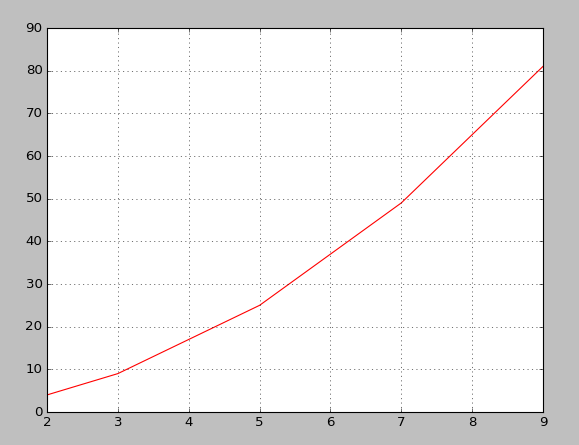
\includegraphics[scale=0.45]{ecran-liste-cours-visualisation-bis}
\end{center}


\begin{lstlisting}
import matplotlib.pyplot as plt

liste_x = [2, 3, 5, 7, 9]
liste_y = [4, 9,25,49,81]
plt.plot(liste_x,liste_y,color="red")
plt.grid()
plt.show()
\end{lstlisting}


\end{document}
